% LaTEX source code
% Last modified November 1st, 2005
% Steve Miller
% note that the percent sign comments out the rest of the line
% first, we set a document class. often use 12pt characters, though
% sometimes people do 11 or 10. you can do report or article, both similar
%\documentclass[12pt,letterpaper]{article}
\documentclass[12pt,reqno]{amsart}
\linespread{1}
\addtolength{\textwidth}{2cm} \addtolength{\hoffset}{-1cm}
\addtolength{\marginparwidth}{-1cm} \addtolength{\textheight}{2cm}
\addtolength{\voffset}{-1cm}
% below are some packages that are needed for certain symbols, graphics, colors.
% safest to just include these.
\usepackage{times}
\usepackage[T1]{fontenc}
\usepackage{mathrsfs}
\usepackage{latexsym}
\usepackage[dvips]{graphics}
\usepackage{epsfig}
\usepackage{hyperref, amsmath, amsthm, amsfonts, amscd, flafter,epsf}
\usepackage{amsmath,amsfonts,amsthm,amssymb,amscd}
\input amssym.def
\input amssym.tex
\usepackage{color}
\usepackage{enumerate}
\usepackage{hyperref}
\usepackage{url}
\usepackage{floatrow}
\usepackage{caption}
\usepackage{subcaption}
\usepackage{capt-of}
\usepackage{physics}
\newcommand{\todo}[1]{\textcolor{red}{\textbf{(#1)}}}

    %=======================================================

    %   THIS IS WHERE YOU PUT SHORTCUT DEFINITIONS

    %========================================================

% Note that we use a percent sign to comment out a line

% below are shortcut commands

%%%%%%%%%%%%%%%%%%%%%%%%%%%%%%%%%%%%%%%%%%%%%%%

% below are shortcuts for equation, eqnarray,

% itemize and enumerate environments

\newcommand\be{\begin{equation}}
\newcommand\ee{\end{equation}}
\newcommand\bea{\begin{eqnarray}}
\newcommand\eea{\end{eqnarray}}
\newcommand\bi{\begin{itemize}}
\newcommand\ei{\end{itemize}}
\newcommand\ben{\begin{enumerate}}
\newcommand\een{\end{enumerate}}
\newcommand{\ncr}[2]{\left({#1 \atop #2}\right)}
%%%%%%%%%%%%%%%%%%%%%%%%%%%%%%%%%%%%%%%%%%%%%%%%

% Theorem / Lemmas et cetera

\newtheorem{thm}{Theorem}[section]
\newtheorem{conj}[thm]{Conjecture}
\newtheorem{cor}[thm]{Corollary}
\newtheorem{lem}[thm]{Lemma}
\newtheorem{prop}[thm]{Proposition}
\newtheorem{exa}[thm]{Example}
\newtheorem{defi}[thm]{Definition}
\newtheorem{exe}[thm]{Exercise}
\newtheorem{rek}[thm]{Remark}
\newtheorem{que}[thm]{Question}
\newtheorem{prob}[thm]{Problem}
\newtheorem{cla}[thm]{Claim}
\newtheorem{defis}[thm]{Definitions}
\newtheorem{res}[thm]{Result}
\newtheorem{calc}[thm]{Calculation}
%%%%%%%%%%%%%%%%%%%%%%%%%%%%%%%%%%%%%%%%%

% shortcuts to environments

% this allows you to do textboldface: simply type \tbf{what you want in bold}

\newcommand{\tbf}[1]{\textbf{#1}}

%%%%%%%%%%%%%%%%%%%%%%%%%%%%%%%%%%%%%%%%%%%%%%%%%%

% shortcut to twocase and threecase definitions

\newcommand{\twocase}[5]{#1 \begin{cases} #2 & \text{#3}\\ #4
&\text{#5} \end{cases}   }
\newcommand{\threecase}[7]{#1 \begin{cases} #2 &
\text{#3}\\ #4 &\text{#5}\\ #6 &\text{#7} \end{cases}   }
%%%%%%%%%%%%%%%%%%%%%%%%%%%%%%%%%%%%%%%%%

%Blackboard Letters

\newcommand{\R}{\ensuremath{\mathbb{R}}}
\newcommand{\C}{\ensuremath{\mathbb{C}}}
\newcommand{\Z}{\ensuremath{\mathbb{Z}}}
\newcommand{\Q}{\mathbb{Q}}
\newcommand{\N}{\mathbb{N}}
\newcommand{\F}{\mathbb{F}}
\newcommand{\W}{\mathbb{W}}
\newcommand{\Qoft}{\mathbb{Q}(t)}  %use in linux
\newcommand{\soln}{\noindent \textbf{Solution:}\ }

%%%%%%%%%%%%%%%%%%%%%%%%%%%%%%%%%%%%%%%%%

% Finite Fields and Groups

\newcommand{\Fp}{ \F_p }
%%%%%%%%%%%%%%%%%%%%%%%%%%%%%%%%%%%%%%%%%

% Fractions

\newcommand{\foh}{\frac{1}{2}}  %onehalf
\newcommand{\fot}{\frac{1}{3}}
\newcommand{\fof}{\frac{1}{4}}

%%%%%%%%%%%%%%%%%%%%%%%%%%%%%%%%%%%%%%%%%

% Legendre Symbols

\newcommand{\js}[1]{ { \underline{#1} \choose p} }

%%%%%%%%%%%%%%%%%%%%%%%%%%%%%%%%%%%%%%%%%

% matrix shortcuts

\newcommand{\mattwo}[4]
{\left(\begin{array}{cc}
                        #1  & #2   \\
                        #3 &  #4
                          \end{array}\right) }
\newcommand{\matthree}[9]
{\left(\begin{array}{ccc}
                        #1  & #2 & #3  \\
                        #4 &  #5 & #6 \\
                        #7 &  #8 & #9
                          \end{array}\right) }
\newcommand{\dettwo}[4]
{\left|\begin{array}{cc}
                        #1  & #2   \\
                        #3 &  #4
                          \end{array}\right| }
\newcommand{\detthree}[9]
{\left|\begin{array}{ccc}
                        #1  & #2 & #3  \\
                        #4 &  #5 & #6 \\
                        #7 &  #8 & #9
                          \end{array}\right| }
%%%%%%%%%%%%%%%%%%%%%%%%%%%%%%%%%%%%%%%%%

% greek letter shortcuts

\newcommand{\ga}{\alpha}                  %gives you a greek alpha
\newcommand{\gb}{\beta}
\newcommand{\gep}{\epsilon}
%%%%%%%%%%%%%%%%%%%%%%%%%%%%%%%%%%%%%%%%%

% general functions

\newcommand{\notdiv}{\nmid}               % gives the not divide symbol
\newcommand{\burl}[1]{\textcolor{blue}{\url{#1}}}

%%%%%%%%%%%%%%%%%%%%%%%%%%%%%%%%%%%%%%%%%%%

% the following makes the numbering start with 1 in each section;

% if you want the equations numbered 1 to N (without caring about

% what section you are in, comment out the following line.

\numberwithin{equation}{section}

%\textwidth= 6in

%\evensidemargin=37pt

%\oddsidemargin=0pt

\begin{document}



\title{Hexane Water Results Log Summer 2018}
\author{Kirk Swanson}
\email{swansonk1@uchicago.edu}
\address{Institute for Molecular Engineering, University of Chicago, 5640 S Ellis Ave, Chicago, IL 60637}
\date{\today}




\maketitle

%%%%%%%%%%%%%%%%%%%%%%%%%%%%%%%%%%%%%%%%%%%%%%%%%%%%%%%%%%%%%%%%%%%%%%%%%%%%%%%%%%%%%%%%%%%%%%%%%%%%%%%%%%%%%%%%%%%%%%%%%%%%%%

\normalsize

%%%%%%%%%%%%%%%%%%%%%%%%%%%%%%%%%%%%%%%%%%%%%%%%%%%%%%%%%%%%%%%%%%%%%%%%%%%%%%%%%%%%%%%%%%%%%%%%%%%%%%%%%%%%%%%%%%%%%%%%%%%%%%
\section{8/6/2018}
\begin{enumerate}
\item Downloaded pressure\_scalar-press-NPT-1bead-water-lammps to dash\_work/interface on laptop.  Used pressure\_analysis\_UPDATE.py leaving out first 2000 records and used 198 blocks 5 ps to get average pressure of 1.41, SE 0.94, SD 511.08: 
\begin{figure}[H]
\centering
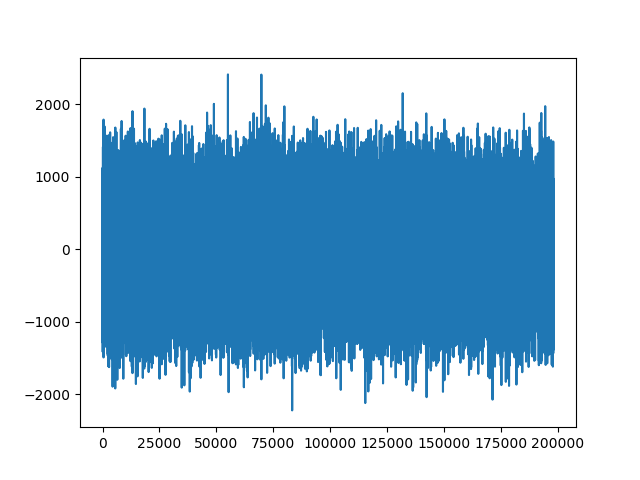
\includegraphics[scale=0.4]{pressures_press-NPT-1bead-water-lammps}
\end{figure}
\item Because we accidentally used restart/traj every 1,000 for fulldata-NPT-298 and then restart/traj 10,000 for fulldata-NPT-298-restart1, we will re-do this calculation again using the updated interface file collecting restart/traj every 1,000.  
\item Submitted simulation no. 1.  
\item To check pressures in a non-vacuum interfacial system, in DASH we are going to run simulation no. 2, which does NPT equilibration for 200,000 steps and then does an NVT simulation of the interface.  Filename press-nonexpanded.
\item Submitted simulation no. 2.  
\item We want to compare the above simulation to LAMMPS, so we will first run the equilibration step in LAMMPS as simulation no. 3.  Note, however, that the mixing rules currently used in the LAMMPS file are arithmetic.  Also NOTE: to use depablo-tc, must type module load openmpi into terminal first, even if it is already in submit script.  After this, we need to run the NVT portion of the simulation for 6M steps.  
\item Running simulation no. 3.
\item Now, let's turn to how pressure is typically computed in DASH.  In general, an ideal gas mechanical equation of state is given by 
\begin{align}
\begin{split}
P = \frac{Nk_BT}{V} = \rho k_BT
\end{split}
\end{align}
This assumes that molecules in the gas are point-like and do not interact with each other.  However, if interactions between the particles and a finite particle volume is allowed.  The virial expansion is a perturbation theory around the ideal gas used when the interactions in the real gas are dominated by two-body interactions.  One uses a virial expansion in powers of the density, keeping the temperature dependence of the coefficients.  We can then apply manipulations of the time derivative of the classical virial to arrive at 
\begin{align}
\begin{split}
P = \rho k_B T - \left[\frac{1}{3V}\left<\sum_{i<j}^Nr_{ij}F_{ij}\right>\right]
\end{split}
\end{align}
where the second term is called the virial correction.  
\item In DASH, it appears as though DataComputerPressure.cu is responsible for scalar pressure values.  On line 92, we have 
\begin{align}
\begin{split}
pressureScalar = (tempScalar\_loc * ndf\_loc * boltz + sumVirial) / (dim * volume) * state->units.nktv\_to\_press
\end{split}
\end{align}
tempScalar\_loc appears to be the temperature of the system, boltz is the boltzmann coefficient, sumVirial is that second virial correction, dim is the dimension of the system.  ndf I calculated to be 3 per atom, including M sites for the water model (printed values using interface file).  So, it does make sense to divide by dim, i.e. divide by 3, because that gets us to N.  However, we are also including M-sites in the pressure value.  So, we are at the very least overcounting the ideal gas term for the pressure.  The amount of overcorrection for 3650 water molecules is given by:
\begin{align}
\begin{split}
P_{c} = \frac{Nk_BT}{V} = \frac{3650\times1.38\times10^{-23}\times 298}{50 \times 10^{-10}\times 50\times 10^{-10}\times 150\times 10^{-10}}
\end{split}
\end{align}
Actually, would it even be incorrect to have four sites per atom?  Maybe that's actually the correct ideal model here?
\end{enumerate}

\section{8/7/2018}
\begin{enumerate}
\item First, we will begin by compiling the most recent version of DASH, which should contain Mike's edits to the TIP4P/F fix for accurate pressure computation (avoiding M-site in ideal gas term).  Compiling version in folder DASH-8-7-2018.  
\item DASH pressure computations:
\subitem NVT with vacuum: run\_UPDATE\_8-7-2018.sh and interface\_UPDATE\_8-7-2018.py, z length 149.2717, x length 58.45467, y length 58.67825, 3650 TIP4P/F water molecules, 500 hexane molecules, waldman-hagler mixing between the water and hexane molecules, NVT with Andersen thermostat with parameters nu = 0.01 (a parameter describing the collision frequency of the system with the heat bath) and applying every 10 steps, 298 K, 1M steps equilibration and 1M steps production, PI false, restart/traj every 10,000, -20/+20 for z change as accounted above, filename newpress-expanded, tensor information commented out in input script. This is simulation no. 4.   
\subitem We will do the same as above, except we will not expand the box by 20 A in each z direction, and we will apply NPT equilibration for 1M steps and then 1M steps of NVT.  This is simulation no. 6.  

\item LAMMPS pressure computations:
\subitem NVT with vacuum: interface.sbatch and in.taffi\_tip4pF\_waldman, x length 149.2717, y length 58.67825, z length 58.45467, 3650 TIP4P/F water molcules, 500 hexane molecules, waldman-hagler mixing, NVT with NoseHoover, 298 K, 1M steps equilibration and 1M steps production, PI false, restart/traj every 10,000, filename newpress-expanded-lammps.  We will start with 500,000 steps and restart from there, which is simulation no. 5. 
\subitem Same as above, except we will not expand the box by 20 A in each z direction, and we will apply NPT equilibration for 1M steps and then 1M steps of NVT.  The first 500,000 steps will be simulation no. 7.  
\subitem Simulation no. 8 is filename newpress-expanded-lammps-restart1, restarting from newpress-expanded-lammps.restart for 1.5M steps 
\subitem Simulation no. 9 is filename newpress-nonexpanded-lammps-restart1, restarting from newpress-nonexpanded-lammps.restart for 500K steps
\subitem Simulation no. 10 is filename newpress-nonexpanded-lammps-restart2, restarting from newpress-nonexpanded-lammps-restart1.restart, and going for 1M NVT steps.  
\end{enumerate}

\section{8/8/2018}
\begin{enumerate}
\item From simulation no. 8, we use pressure\_analysis\_UPDATE.py on laptop in dash\_work/interface folder to analyze pressures\_scalar-newpress-expanded-lammps-restart.txt.  We use indices 50,000 to 150,000 and 100 SE blocks of size 5 ps.  This gives us a mean pressure of -83.443 atm, SE of the mean 1.578 atm, and SD of the distribution 154.699 atm.  Here is a plot of these values over time:
\begin{figure}[H]
\centering
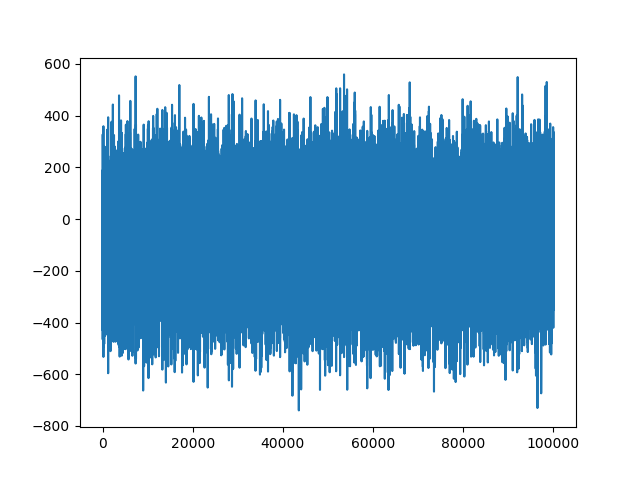
\includegraphics[scale=0.7]{pressures_newpress-expanded-lammps-restart1}
\end{figure}
\item From simulation no. 4, we use pressure\_analysis\_UPDATE.py on laptop in dash\_work/interface to analyze pressure\_scalar-newpress-expanded.txt.  We use indices 100,000 to 200,000 and 100 SE blocks of size 5 ps.  This gives us a mean pressure of -70.603 atm, SE of the mean 1.487 atm, and SD of the pressures 154.854.  Here is a plot:
\begin{figure}[H]
\centering
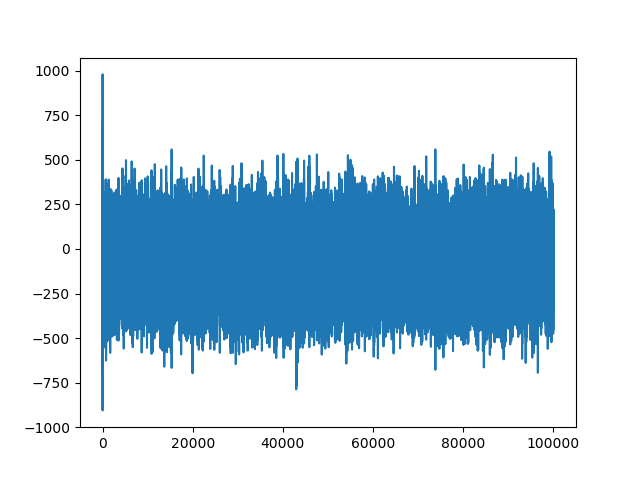
\includegraphics[scale=0.7]{pressures_newpress-expanded}
\end{figure}
Removing the first 100 values for better comparison to the above plot, we have:
\begin{figure}[H]
\centering
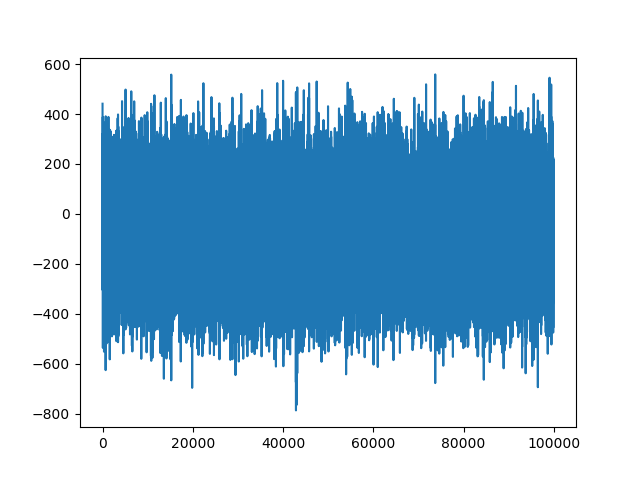
\includegraphics[scale=0.7]{pressures_newpress-expanded-clipped}
\end{figure}
\item If we combine pressures\_scalar-newpress-expanded-lammps.txt and pressures\_scalar-newpress-expanded-lammps-restart1.txt, then we have all 2M steps covered.  We call this file pressures\_scalar-newpress-expanded-lammps-combined.txt.  Analyzing all points in this file, using 200 blocks of size 5 ps, we get an average pressure of -80.945, SE of the mean 1.237, and SD of values 156.056:
\begin{figure}[H]
\centering
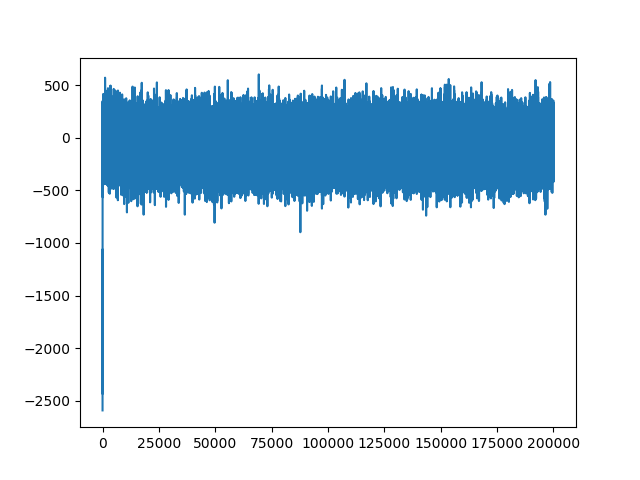
\includegraphics[scale=0.7]{pressures_newpress-expanded-lammps-combined}
\end{figure}
\item Using all values from pressures\_scalar-newpress-expanded.txt from DASH, using 200 blocks as well, we get a mean pressure of -77.716, SE of the mean 1.337, and SD of values 155.610:
\begin{figure}[H]
\centering
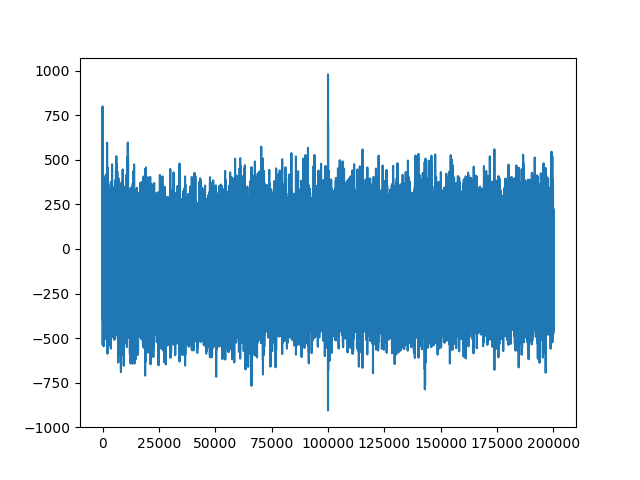
\includegraphics[scale=0.7]{pressures_newpress-expanded-full}
\end{figure}
\item Andersen Thermostat: Rescales velocities at regular timesteps to control the temperature
\item NoseHoover Thermostat: Integrates equations of motion derived from a Hamiltonian that has an extra degree of freedom for the heat bath
\item From simulation no. 6, in DASH, we did 1M NPT steps followed by 1M NVT steps so that we can analyze pressure from the NVT which will not have vacuum, in theory.  The box dimensions we get from this simulation are: x length 48.875, y length 49.061, z length 91.3641.  Downloading pressure\_scalar-newpress-nonexpanded.txt to dash\_work/interface on laptop for analysis as above.  Using the 1M NPT plus 1M NVT data and 200 blocks, we have a mean pressure of -31.943, SE of the mean 3.174, and SD of values 333.460:
\begin{figure}[H]
\centering
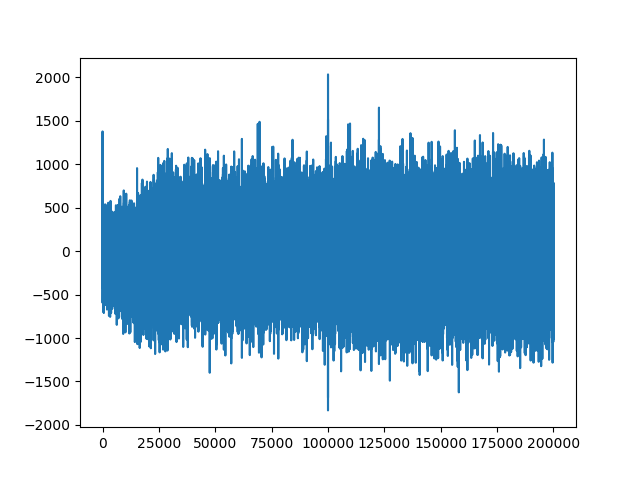
\includegraphics[scale=0.7]{pressures_newpress-nonexpanded-full}
\end{figure}
Using only the 1M NVT steps, and 100 blocks, we have a mean pressure of -32.501, SE of the mean 3.592, SD of values 364.244:
\begin{figure}[H]
\centering
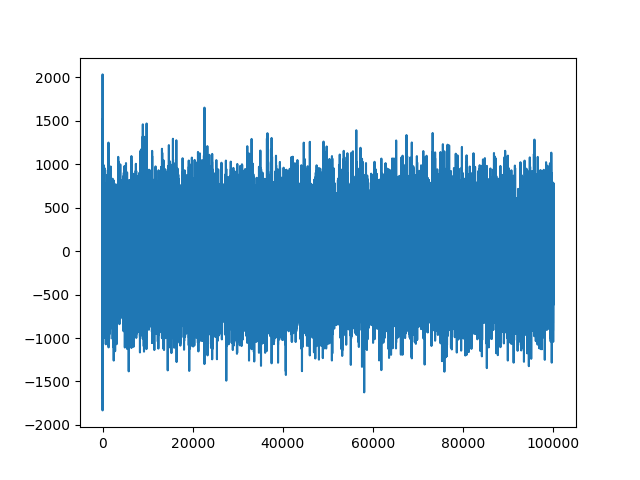
\includegraphics[scale=0.7]{pressures_newpress-nonexpanded}
\end{figure}
\item From simulation no. 10, in LAMMPS, we did 1M NVT steps after 1M NPT equilibration.  The box dimensions are: x length 90.498, y length 48.597, z length 48.412.  These lengths are slightly different from the above DASH simulation.  The NVT component of the simulation, from pressures\_scalar-newpress-nonexpanded-lammps-restart2.txt, we get a mean pressure of 54.504, SE of the mean 4.47, and SD of values 375.729, using 100 blocks:
\begin{figure}[H]
\centering
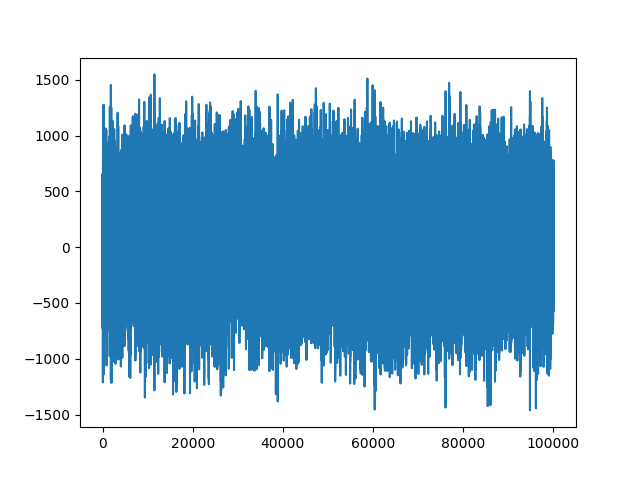
\includegraphics[scale=0.7]{pressures_newpress-nonexpanded-lammps-restart2}
\end{figure}
Combining the NPT steps into pressures\_scalar-newpress-nonexpanded-lammps-combined.txt, we get a mean pressure of 25.947, SE 3.152, and SD 374.379 using 200 blocks: 
\begin{figure}[H]
\centering
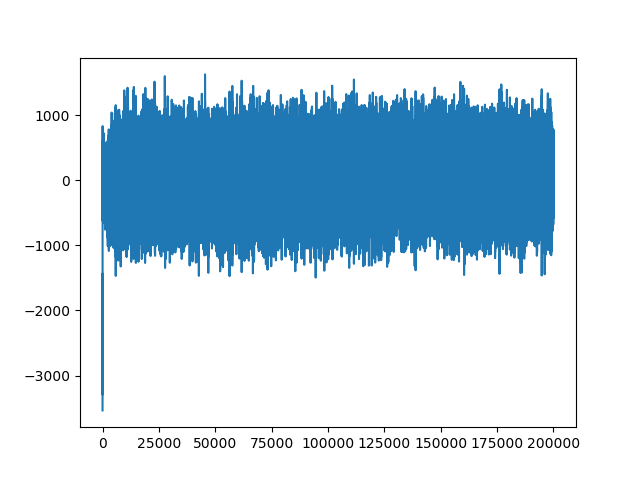
\includegraphics[scale=0.7]{pressures_newpress-nonexpanded-lammps-combined}
\end{figure}
\item It is possible that we have differing values here because the volumes are slightly different.  To test the hypothesis that the vacuum is responsible for the negative pressure, let's try decreasing the volume by only putting 10 Angstroms on each side of the simulation box.  
\item Simulation no. 11 in DASH will take care of this filename newpress-smallexpanded, and simulation no. 12 in LAMMPS will do the same. 
\item Simulation no. 13 will be DASH 2M NPT of the interface
\item Simulation no. 14 will be LAMMPS NPT of the interface
\item Simulation no. 15 will be DASH 2M NVT at 0.997 of TIP4P/F 3650 molecules
\item Simulation no. 16 will be 2M NPT at 1 atm of 3650 molecules in DASH
\end{enumerate}


\section{8/9/2018}
\begin{enumerate}
\item 
\begin{figure}[H]
\centering
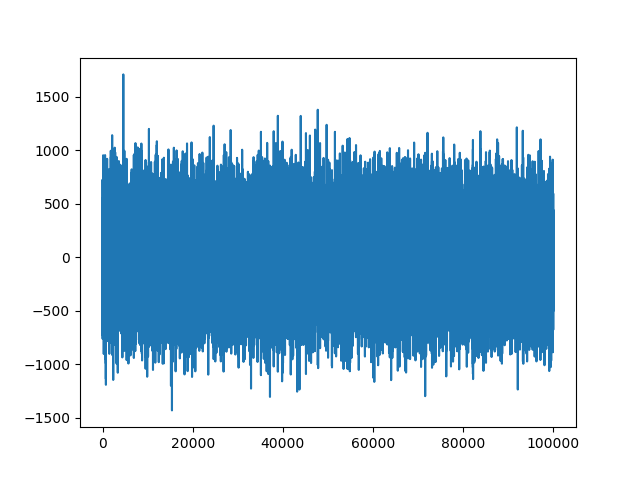
\includegraphics[scale=0.7]{pressures_newpress-NPT}
\end{figure}
\begin{figure}[H]
\centering
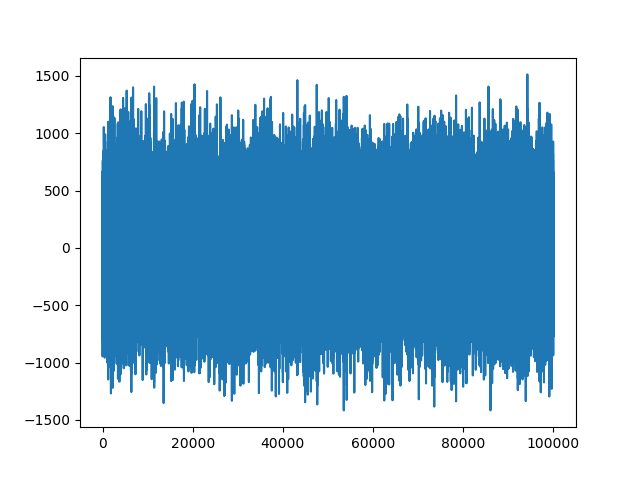
\includegraphics[scale=0.7]{pressures_newpress-NPT-lammps}
\end{figure}
\end{enumerate}

\section{8/11/2018}
\begin{enumerate}
\item First, we need to re-do molecular orientation plots.  The file molecular\_orientation\_water\_postproduction\_UPDATE.py contains the unwrap update that is necessary for accurate analysis.  In this file, we correctly unwrap molecules based on the location of the oxygen atom.  In dash\_work/interface on Midway, we will use orientation\_postproduction.sbatch to do water orientation postproduction profiles from the 1bead trajectory, full-298-1bead, and the 32 bead trajectory, full-298-32bead-combined.xyz.  The filename for 1bead is orientations\_water\_unwrap.txt, which once downloaded to laptop was copied as orientations\_water\_full-298-1bead-orientations-water.txt.  The filename for 32bead is orientations\_water\_32bead-water-unwrap.txt.    
\item For full-298-1bead, we used indices 600 to 960:
\begin{figure}[H]
\centering
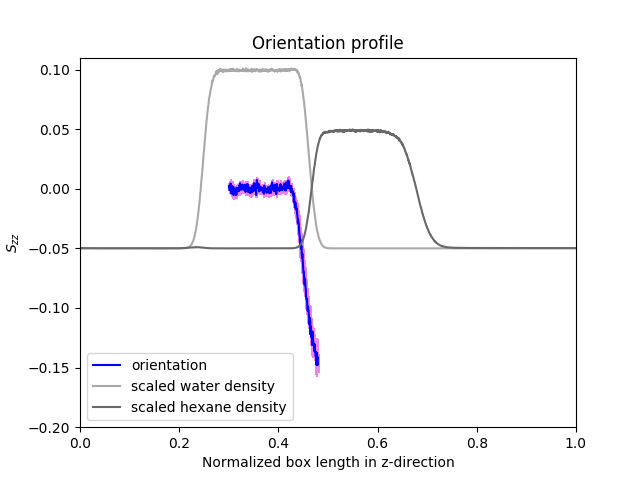
\includegraphics[scale=0.7]{full-298-1bead-orientations-water-corrected}
\end{figure}
\item We also corrected molecular\_orientation\_hexane\_postproduction\_UPDATE.py to have the appropriate unwrapping procedure.  We use this in orientation\_postproduction\_hexane.sbatch to analyze the same trajectory files as above for hexane.  The 1bead file is orientations\_hexane\_full-298-1bead-orientations-hexane-corrected.txt.  We download this onto laptop and use indices 900 to 1150 to obtain:
\begin{figure}[H]
\centering
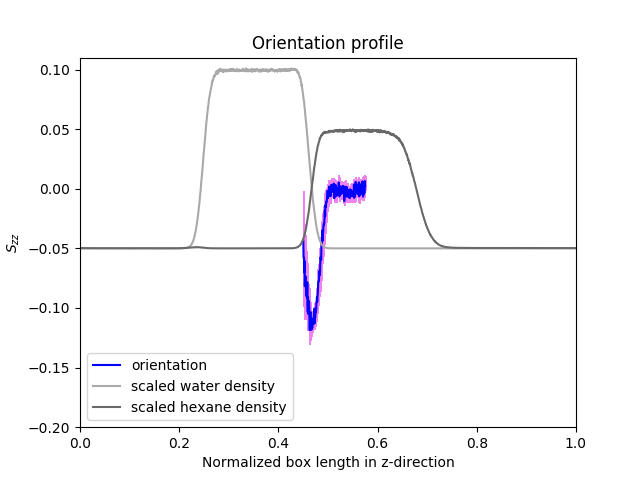
\includegraphics[scale=0.7]{full-298-1bead-orientations-hexane-corrected}
\end{figure}
We are also running the 32 bead version, named as above, orientations\_hexane\_full-298-32bead-orientations-hexane-corrected.txt.
\item We recently resolved the negative pressure issue.  Let's start from Section 2.5 of The Molecular Theory of Capillarity, by J. S. Rowlinson and B. Widom.  The assumption we begin with is that it is possible to consistently define local values of the thermodynamic fields $p, T, \mu$ even in an inhomogeneous system.  At a planar fluid-fluid interface, confied to a cube of sidelength l and interfacial area A = $l^2$, these fields and densities are functions only of the z dimension, defined as normal to the interfacial plane.  We call the pressure in either bulk phase the scalar quantity $p$.  Near the interface the pressure is a tensor since its tangential components, parallel with a dividing surface, include the tension of the interface, and so differ from the normal component.  Mechanical stability requires that the gradient of this tensor is zero everywhere in the fluid, $\triangledown \cdot \vec{p} = 0$ , and the symmetry of the surface requires that $\vec{p}$ is a diagonal tensor, $\vec{p}(\vec{r}) = p_{xx}(\vec{r})e_xe_x + p_{yy}(\vec{r})e_ye_y + p_{zz}(\vec{r})e_ze_z$ with $p_{xx}(\vec{r}) = p_{yy}(\vec{r})$.  Substitution of this equation into the gradiant equation yields $p_{zz}(z) = p_{yy}(z) = p_T(z)$ and $p_{zz}(z) = p_N(z) = p$, where $p_N$ and $p_T$ are the normal and transverse components of the pressure.  If a side-wall of the cube is displaced isothermally and reversibly so as to increase the area by $\delta A$, then the tengential work done on the system is $\delta W_T = -\delta A\int_{-l/2}^{l/2}p_T(z)dz$.  A similar displacement of the top or bottom wall by a distance $\delta A / l$ serves to maintain the volume constant, and requires further (normal) work $\delta W_N = A(\delta A/l)p = l\delta Ap$.  Thus, the total work done, and hence the increase in free energy, is $\delta F = \delta W_T + \delta W_N = \delta A\int_{l/2}^{l/2}[p - p_T(z)]dz$.  Using $dF = -SdT - pdV + \gamma dA + \mu dN$.  So, we can associate this integral with the interfacial tension.    
\item This brings us to the following.  We define the interfacial tension as $\gamma = \int_0^{L_z}[p_N(z) - p_T(z)]dz$.  Since at a stable planar interface the gradiant of the pressure tensor must be zero, the tensor must be symmetric, and the bulk pressures have scalar value $p$, we can define $p_N(z) = p_{zz} = p$ and $p_T(z) = \frac{p_{xx}(z) + p_{yy}(z)}{2}$.  Using the mean value theorem, we can write the average pressure tensor elements obtained from an MD simulation, $<p_{xx}> = p_{xx}$ and $<p_{yy}> = p_{yy}$ as $p_{xx} = \frac{1}{L_z}\int_0^{L_z}p_{xx}(z)dz$ and $p_{yy} = \frac{1}{L_z}\int_0^{L_z}p_{yy}(z)dz$.  We can then carry out the integration that defines $\gamma$ and rewrite the interfacial tension as $\gamma = (p - \frac{p_{xx} + p_{yy}}{2})$, which is the standard formula for computing interfacial tension in molecular simulations.  In our simulation box, we have two interfaces, so the interfacial tension associated with a single interface can be given by dividing by two:  $\gamma = \frac{1}{2}(p - \frac{p_{xx} + p_{yy}}{2})$.  We assume that the bulk phases are at their equilibrium densities corresponding to $p \approx 1 \text{ atm }$, either by measuring the bulk densities in an NVT simulation or by applying a barostat in the z dimension to maintain $p \approx 1 \text{ atm }$.  For hexane-water, the experimental interfacial tension is 50 $\frac{mN}{m} = 4, 900 \text{atm}\cdot $\AA.  Our simulation box is approximately 100 \AA in the z dimension, so, we have 4,900 atm $\cdot$ \AA = (1 atm - $\frac{p_{xx} + p_{yy}}{2})\cdot$ 100 \AA.  We can solve this to get $p_{xx} + p_{yy} = -194$.  Since the scalar pressure in an MD simulation is computed as $P_{tot} = \frac{p_{xx} + p_{yy} + p_{zz}}{3}$, we have $P_{tot} = -64.33$.  What happens to these negative scalar pressures in the thermodynamic limit?  In ambient conditions, $\gamma$ would still be 50 $\frac{mN}{m}$ and $p = 1 \text{ atm }$, but $L_z\rightarrow\infty$, so $\text{lim}_{L_z\rightarrow\infty}\frac{\gamma}{L_z} = 0$, which implies that $\frac{p_{xx} + p_{yy}}{2}$ converges to $p$ and $P_{tot} \rightarrow 1$. 
\begin{align}
\begin{split}
\gamma = \int_{0}^{L_z}[p_N(z) - p_T(z)]dz
\end{split}
\end{align} 
\begin{align}
\begin{split}
p_N(z) = p_{zz} = p
\end{split}
\end{align} 
\begin{align}
\begin{split}
p_T(z) = \frac{p_{xx}(z) + p_{yy}(z)}{2}
\end{split}
\end{align} 
\begin{align}
\begin{split}
= \frac{1}{2}\left(p - \frac{p_{xx} + p_{yy}}{2}\right)L_z
\end{split}
\end{align} 
\begin{align}
\begin{split}
p_{xx} = \left<p_{xx}(z)\right> = \frac{1}{L_z}\int_{-L_z/2}^{L_z/2}p_{xx}(z)dz
\end{split}
\end{align} 
\begin{align}
\begin{split}
4,900 \text{ atm } \text{\AA} \approx (1 \text{ atm } - \frac{p_{xx} + p_{yy}}{2})\cdot 100 \text{\AA}
\end{split}
\end{align} 
\begin{align}
\begin{split}
p_{xx} + p_{yy} \approx -194
\end{split}
\end{align} 
\begin{align}
\begin{split}
P_{\text{tot, MD sim.}} = \frac{p_{xx} + p_{yy} + p_{zz}}{3} \approx -65\text{ atm}
\end{split}
\end{align}
\begin{align}
\begin{split}
\text{lim}_{L_z\rightarrow\infty}\frac{\gamma}{L_z}\rightarrow = 0
\end{split}
\end{align} 
\begin{align}
\begin{split}
\frac{p_{xx} + p_{yy}}{2} \rightarrow p
\end{split}
\end{align} 
\end{enumerate}

\section{8/12/2018}
\begin{enumerate}
\item Working on slides explaining capillary theory contributions for candidacy ppt.  
\item We download orientations\_hexane\_full-298-32bead-hexane-orientations-corrected.txt and analyzed:
\begin{figure}[H]
\centering
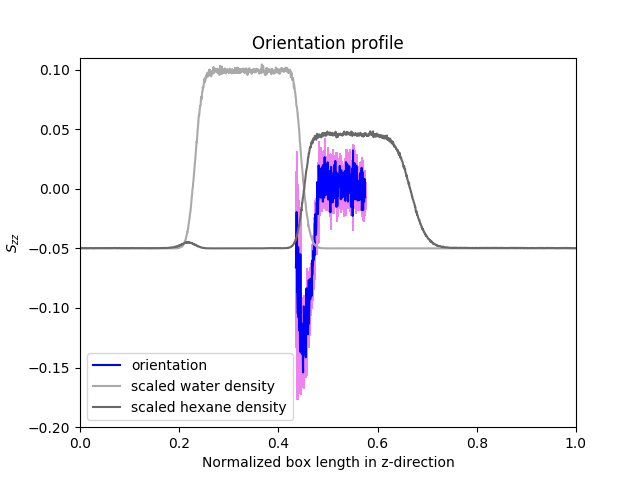
\includegraphics[scale=0.7]{full-298-32bead-orientations-hexane-corrected}
\end{figure}
\item Download orientations\_water\_32bead-water-unwrap.txt.  Had issues with nan in orientation\_profile\_analysis\_UPDATE for some strange reason, nans in the SE measurements, so used nan\_policy='omit' for stats.sem.  Finally, it works: used zlo 600 zhi 940:
\begin{figure}[H]
\centering
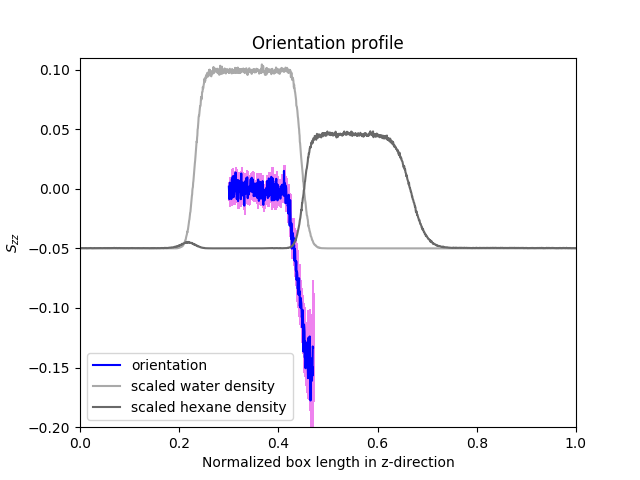
\includegraphics[scale=0.7]{full-298-32bead-orientations-water-corrected}
\end{figure}
\end{enumerate}


\end{document}